\documentclass[11pt,a4paper]{article}
\usepackage[margin=2.4cm]{geometry}
\usepackage[T1]{fontenc}
\usepackage[utf8]{inputenc}
\usepackage[french]{babel}
\usepackage{booktabs}
\usepackage{graphicx}
\usepackage{hyperref}
\usepackage{amsmath}

\title{Etude de sensibilite des parametres -- rapport preliminaire}
\author{modele-27-04-WIP / studies/sensitivity}
\date{27 avril 2026}

\begin{document}
\maketitle

\section{Statut et principe}

Ce document est un rapport preliminaire, pas le rapport final. Il fixe les
premiers resultats robustes avant la grande campagne OAT et les couplages.
Le cadre corrige est le suivant : les simulations principales sont homogenes
au sens \(\alpha_{\min}=\alpha_{\max}=1\), mais
\(\sigma_\alpha=\) \texttt{alpha\_sigma\_brownien} est maintenant un parametre
de sensibilite. L'amortissement reste fixe a zero.

Le premier critere utilise dans les scripts cherchait une chute conjointe forte
de \(n_{\mathrm{alive}}\) et de l'actif. Il etait trop restrictif. Le regime
permanent doit plutot etre compris comme une dynamique bornee apres un temps
fini : les stocks restent dans une plage finie, meme si la chute initiale est
faible, par exemple 5\%, ou meme si l'actif et le nombre d'entites deviennent
partiellement decorreles. Les nouveaux diagnostics utilisent donc :
\begin{itemize}
  \item la premiere chute de \(n_{\mathrm{alive}}\) de 5\% comme repere visuel ;
  \item les pentes relatives en queue de \(n_{\mathrm{alive}}\), de l'actif et
  de la densite financiere ;
  \item la pente des faillites en queue, pour detecter un regime encore en train
  de se former ;
  \item les correlations de queue entre \(n_{\mathrm{alive}}\), actif total et
  reseau de prets.
\end{itemize}

\section{Premier point critique : \(k\) et conditions d'apparition du regime}

Le point central strictement homogene avec \(k=3\) et
\(\sigma_\alpha=0\) ne donne pas de regime dans les tests a 1000--2000 pas.
Le pilote baseline a produit 0 convergence sur 5 seeds a 1000 pas, et la sonde
guidee par \texttt{simulation\_lab} confirme qu'a 2000 pas, \(k=3\) reste dans
une croissance de population et un reseau peu dense.

En revanche, \(k=3\) atteint un regime permanent lorsque
\(\sigma_\alpha\) est non nul : une volatilite brownienne moderee de
productivite suffit a amorcer les cascades et a creer le reseau dense.
Le tableau de la section~\ref{sec:sigma} donne la fenetre active
\(\sigma_\alpha\in[0.005,0.02]\).

Le passage a \(k=4\) simplifie l'apparition du regime : il est present des
\(\sigma_\alpha=0\) et reste robuste jusqu'a \(\sigma_\alpha\approx0.02\).
Le parametre \(k=\) \texttt{n\_candidats\_pool} n'est donc pas un simple
parametre d'intensite continue : il controle la facilite avec laquelle le
regime apparait, et agit comme un parametre de bifurcation autour du point
central homogene statique (\(\sigma_\alpha=0\)).

\section{Choix numerique : epsilon}

Un benchmark a compare \(\epsilon\in\{10^{-6},10^{-5},10^{-4},10^{-3},10^{-2}\}\)
sur deux regimes representatifs : homogene \(k=4\) et heterogene \(k=3\).
Le resultat est net :

\begin{itemize}
  \item \(\epsilon=10^{-2}\) change qualitativement le modele : le regime dense
  disparait et la densite financiere tombe vers \(0.006\)--\(0.009\).
  \item \(\epsilon=10^{-3}\) conserve la densite financiere a quelques pourcents
  pres, tout en accelerant fortement les simulations.
  \item le nombre de contrats par entite depend beaucoup de \(\epsilon\). Cette
  metrique doit donc etre interpretee comme une metrique de resolution du reseau
  autant que comme une metrique economique.
\end{itemize}

Decision provisoire : utiliser \(\epsilon=10^{-3}\) comme valeur par defaut
pour cartographier l'espace des parametres rapidement. Si un point ne produit
pas de convergence vers un regime a \(\epsilon=10^{-3}\), on teste
\(\epsilon=10^{-4}\) puis \(\epsilon=10^{-6}\) avant de conclure a l'absence
de regime : une valeur trop grossiere peut empecher artificiellement la
formation du reseau dense (voir section~\ref{sec:k}). Les points de reference
et le nombre de contrats par entite sont mesures a \(\epsilon=10^{-6}\).

Cette observation a une interpretation importante : \(\epsilon\) ne semble pas
modifier le volume de credit tant qu'il reste sous un seuil, mais il modifie
fortement le nombre de contrats. Cela indique que le reseau contient beaucoup de
micro-credits. Pour les statistiques de cascades, cette granularite peut etre
decisive : deux simulations ayant le meme volume de credit peuvent avoir des
topologies de contagion differentes si l'une remplace de nombreux micro-liens
par moins de liens effectifs.

\begin{figure}[ht]
  \centering
  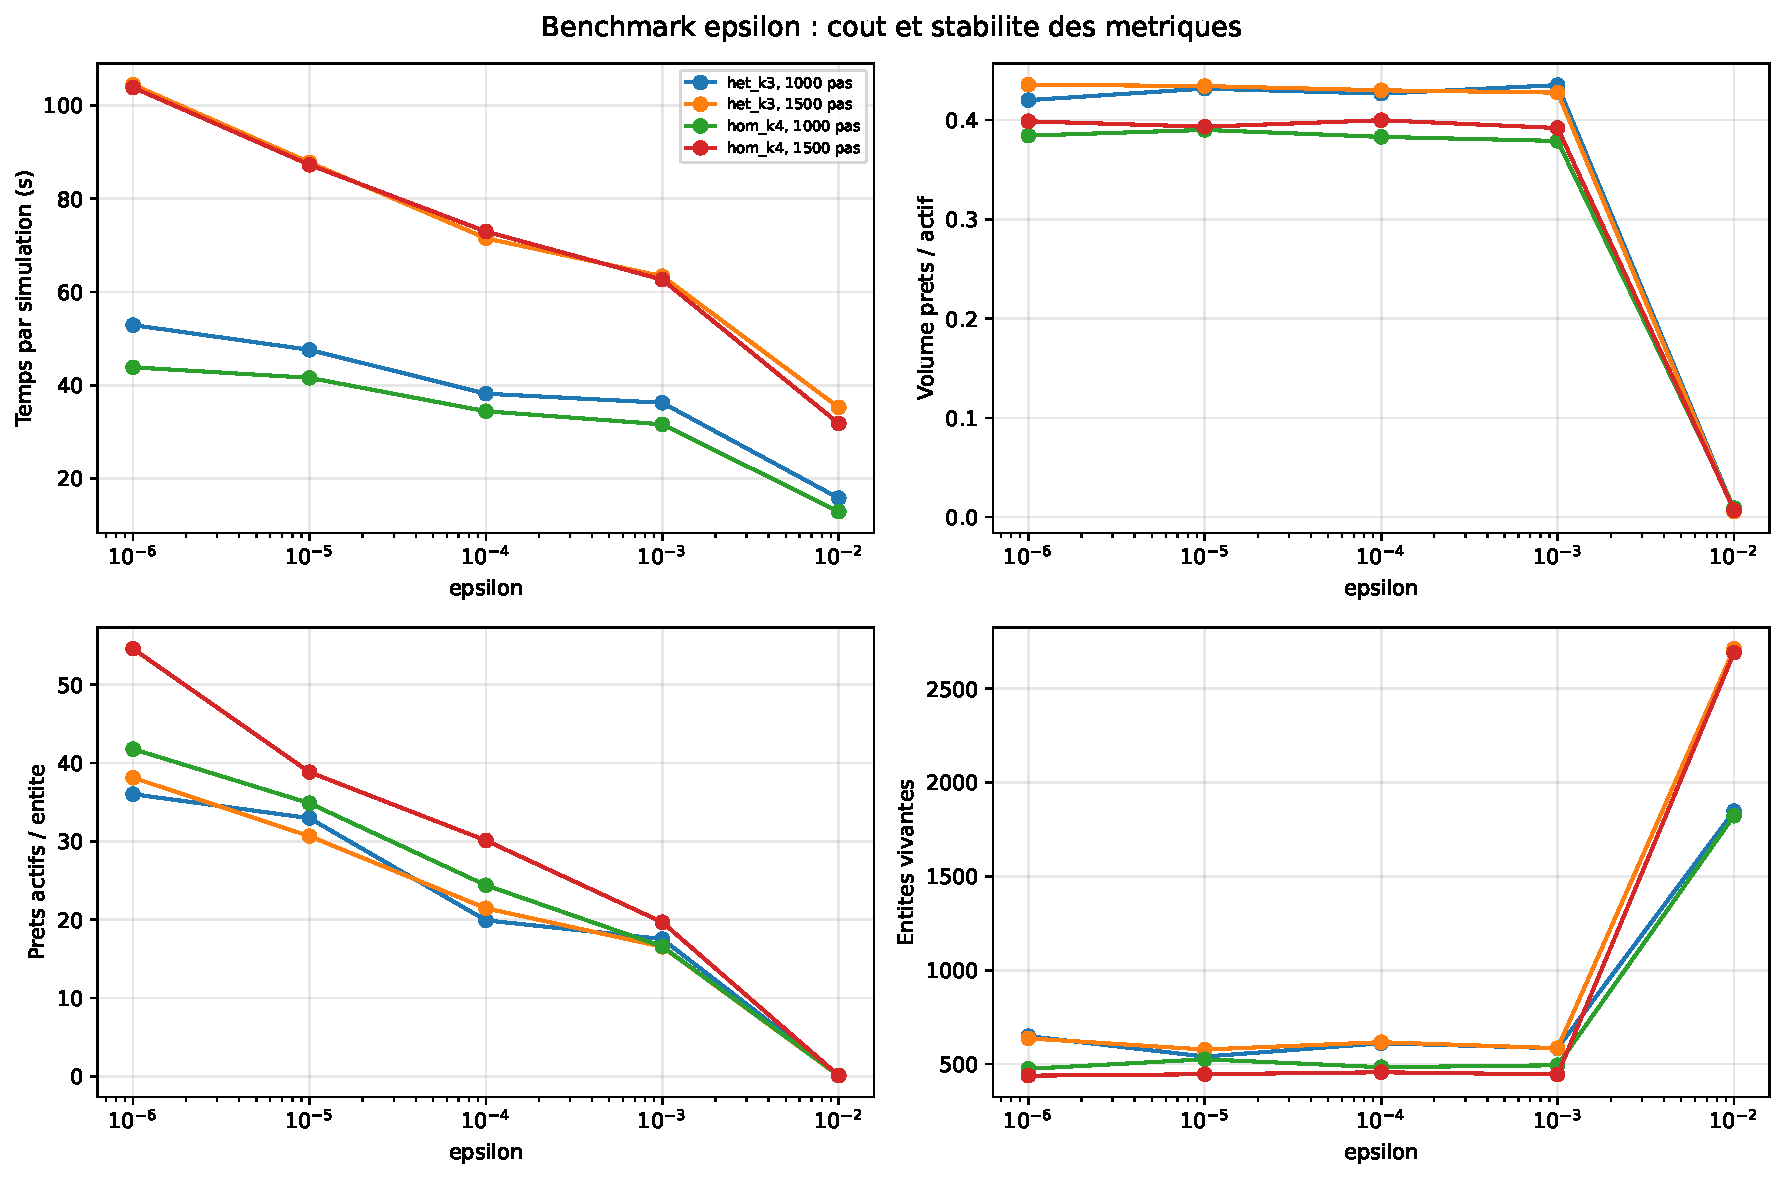
\includegraphics[width=0.95\linewidth]{figures/epsilon_runtime_probe.pdf}
  \caption{Compromis cout / stabilite des metriques lorsque \(\epsilon\) varie.}
\end{figure}

\section{Balayage de \(k\) et plateau}
\label{sec:k}

Le balayage de \(k\) a ete fait a \(\epsilon=10^{-3}\), 1500 pas, avec trois
seeds sur les valeurs critiques et de plateau. Les valeurs larges de \(k\)
testent explicitement l'hypothese d'un plateau.

La lecture correcte est une lecture a seuil. Pour \(k\) trop faible, le marche
du credit ne cree pas de reseau dense : les volumes financiers restent faibles
et les naissances ne sont pas compensees par une mortalite endogene suffisante.
Une fois le seuil franchi, le reseau se forme brutalement. Augmenter encore
\(k\) ne produit pas une croissance indefinie de la densite financiere : on
observe plutot un plateau. Ce comportement est analogue a celui observe pour
\(\epsilon\), mais avec une difference essentielle : \(k\) est un parametre du
mecanisme economique de rencontre, tandis qu'\(\epsilon\) est une resolution
numerique qui peut empecher artificiellement la creation du regime si elle est
trop grossiere.

\begin{table}[ht]
\centering
\begin{tabular}{lrrrr}
\toprule
Scenario & \(k\) & part regime & densite financiere & prets / entite \\
\midrule
homogene & 2  & 0/3 & 0.015 & 0.22 \\
homogene & 3  & 0/3 & 0.049 & 0.71 \\
homogene & 4  & 3/3 & 0.399 & 21.27 \\
homogene & 5  & 3/3 & 0.411 & 26.92 \\
homogene & 8  & 3/3 & 0.381 & 23.42 \\
homogene & 20 & 3/3 & 0.380 & 25.30 \\
homogene & 50 & 3/3 & 0.375 & 23.19 \\
\midrule
heterogene & 2  & 0/3 & 0.092 & 1.52 \\
heterogene & 3  & 3/3 & 0.429 & 16.41 \\
heterogene & 4  & 2/3 & 0.464 & 27.60 \\
heterogene & 5  & 3/3 & 0.477 & 36.43 \\
heterogene & 8  & 3/3 & 0.501 & 57.14 \\
heterogene & 20 & 3/3 & 0.509 & 55.81 \\
heterogene & 50 & 1/3 & 0.446 & 35.75 \\
\bottomrule
\end{tabular}
\caption{Balayage de \(k\), 1500 pas, \(\epsilon=10^{-3}\).}
\end{table}

\begin{figure}[ht]
  \centering
  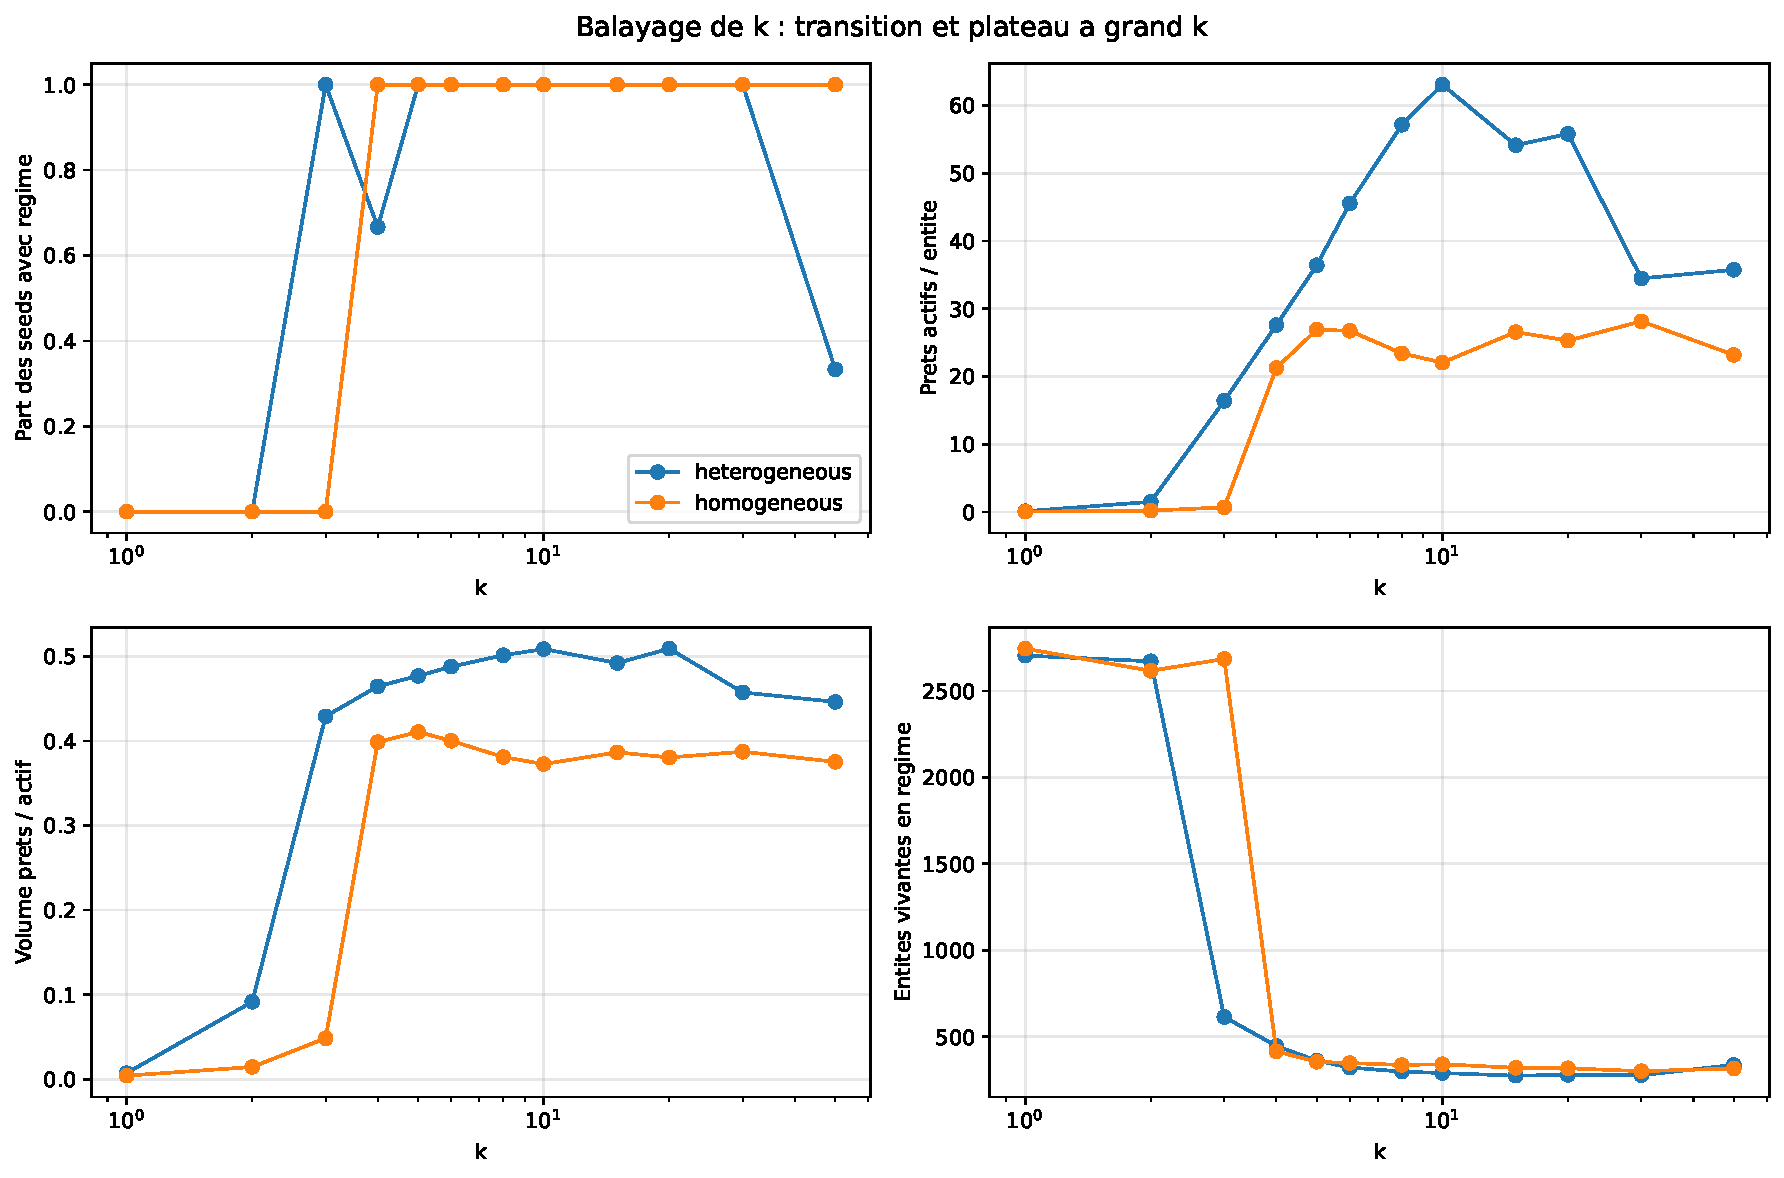
\includegraphics[width=0.95\linewidth]{figures/k_sweep_steps1500_eps0.001.pdf}
\caption{Transition et plateau lorsque \(k\) augmente.}
\end{figure}

\section{Cas temoin : regime sans chute conjointe detectee}

Le run \texttt{20260427\_145524\_ff4328fa} du \texttt{simulation\_lab}
illustre pourquoi le critere de chute conjointe etait insuffisant. Ses
parametres sont homogenes a la naissance,
\(\alpha_{\min}=\alpha_{\max}=1\), avec \(\sigma_\alpha=0.05\),
\(k=4\) et \(\epsilon=10^{-3}\). L'ancien scan l'avait classe
\texttt{no\_joint\_drop}. Pourtant, en fin de simulation, il est clairement dans
une dynamique bornee : entre les pas 1990 et 1999, \(n_{\mathrm{alive}}\) reste
autour de 531--540, l'actif total autour de \(5.66\times10^7\), et le volume de
prets autour de \(5.1\times10^6\).

Ce cas est aussi interessant parce que \(n_{\mathrm{alive}}\) et l'actif total
ne portent pas la meme information. Sur les queues longues, la correlation
\(\mathrm{corr}(n_{\mathrm{alive}}, A)\) varie fortement selon la fenetre :
elle vaut environ \(0.36\) apres le pas 1000, devient presque nulle apres le pas
1200, puis negative sur les queues plus tardives. Autrement dit, le nombre
d'entites peut etre stationnaire pendant que la taille moyenne et la structure
financiere des entites survivantes evoluent encore. La taille du systeme doit
donc etre analysee au moins avec deux variables, \(n_{\mathrm{alive}}\) et
actif total, et pas seulement par leur correlation brute.

\section{Volatilite brownienne en alpha homogene}
\label{sec:sigma}

La correction importante est la suivante : l'analyse principale reste homogene
en niveau initial, \(\alpha_{\min}=\alpha_{\max}=1\), mais
\(\sigma_\alpha\) varie. Il ne s'agit donc pas de comparer directement une
population initialement heterogene a une population homogene ; on teste plutot
la capacite d'une volatilite dynamique de productivite a creer ou detruire le
regime.

\begin{table}[ht]
\centering
\begin{tabular}{rrrrrr}
\toprule
\(k\) & \(\sigma_\alpha\) & queue bornee & densite fin. & prets/entite & taille cascade \\
\midrule
3 & 0     & 0/3 & 0.050 & 0.73  & 1.00 \\
3 & 0.003 & 0/3 & 0.094 & 1.36  & 1.04 \\
3 & 0.005 & 1/3 & 0.348 & 6.40  & 4.03 \\
3 & 0.010 & 2/3 & 0.429 & 15.51 & 2.45 \\
3 & 0.020 & 2/3 & 0.489 & 25.66 & 2.18 \\
3 & 0.050 & 0/3 & 0.053 & 21.73 & 1.59 \\
3 & 0.100 & 0/3 & 0.001 & 12.01 & 1.57 \\
\midrule
4 & 0     & 3/3 & 0.401 & 21.89 & 2.38 \\
4 & 0.005 & 3/3 & 0.443 & 24.67 & 2.29 \\
4 & 0.020 & 3/3 & 0.520 & 43.10 & 2.36 \\
4 & 0.050 & 0/3 & 0.131 & 94.14 & 2.39 \\
4 & 0.100 & 0/3 & 0.001 & 36.85 & 2.06 \\
\bottomrule
\end{tabular}
\caption{Effet de \(\sigma_\alpha\) avec \(\alpha_{\min}=\alpha_{\max}=1\), \(\epsilon=10^{-3}\), 1500 pas.}
\end{table}

\begin{figure}[ht]
  \centering
  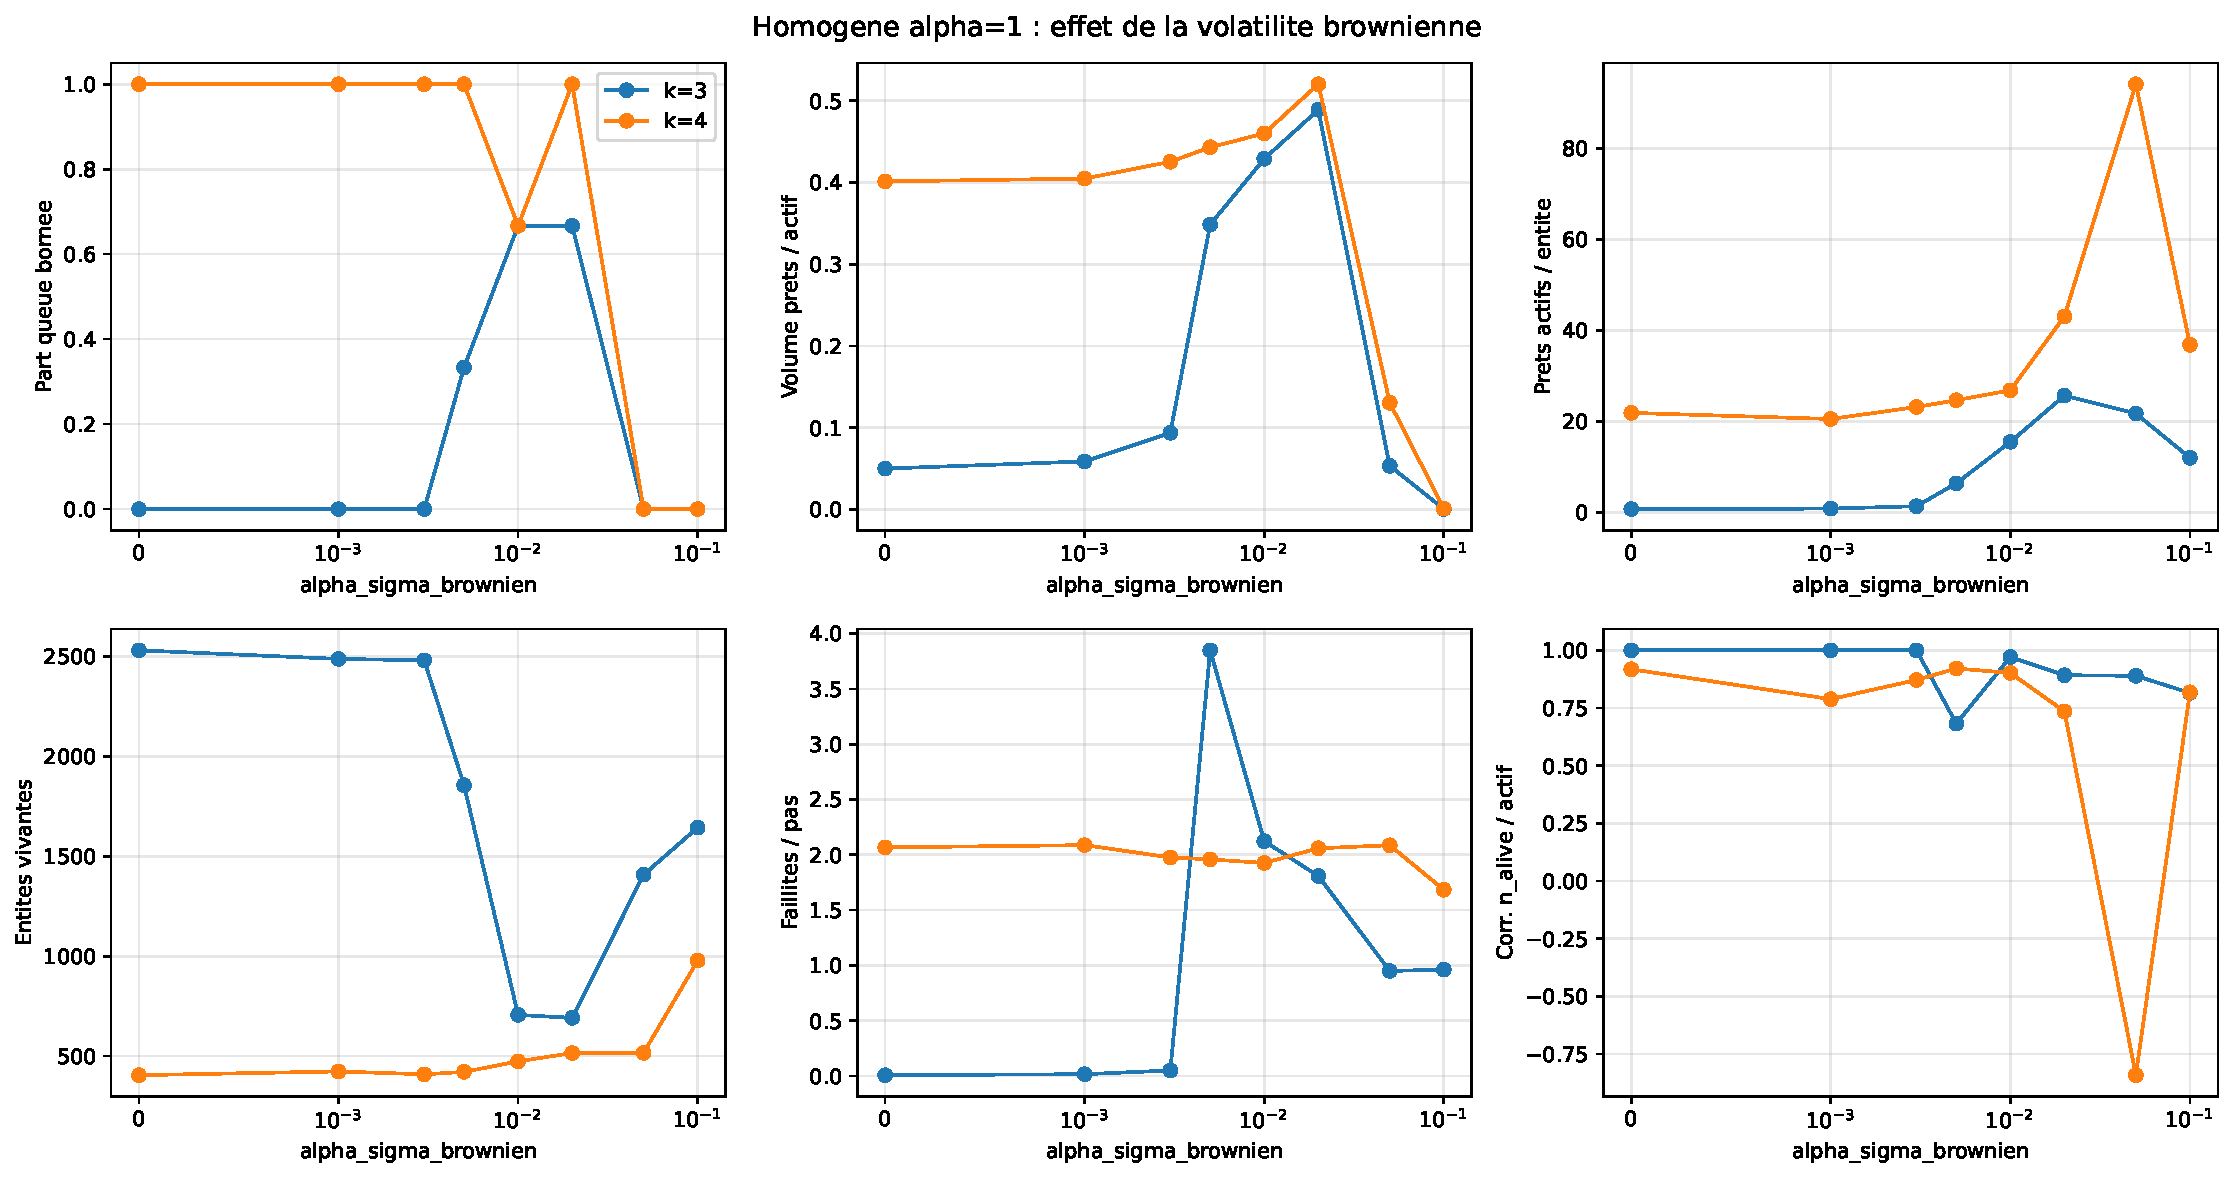
\includegraphics[width=0.95\linewidth]{figures/alpha_sigma_sweep_steps1500_eps0.001.pdf}
  \caption{Fenetre active de volatilite brownienne en alpha homogene.}
\end{figure}

Deux faits ressortent. Pour \(k=3\), une volatilite trop faible ne suffit pas a
creer le reseau dense ; une volatilite intermediaire, environ
\(\sigma_\alpha=0.005\)--\(0.02\), fait apparaitre le regime ; une volatilite
trop forte detruit a nouveau le volume financier. Pour \(k=4\), le regime est
deja present a \(\sigma_\alpha=0\), puis la volatilite augmente le volume de
credit jusqu'a \(\sigma_\alpha\approx0.02\). A \(\sigma_\alpha=0.05\), le
nombre de contrats par entite devient tres eleve mais le volume financier
retombe, ce qui indique une fragmentation en nombreux micro-credits et une
decorrélation plus forte entre population et actif.

\section{Interpretation provisoire}

Trois faits structurent la suite de l'etude.

Premierement, dans le modele strictement statique
(\(\alpha_{\min}=\alpha_{\max}=1\), \(\sigma_\alpha=0\)), \(k=3\) est
sous-critique : le reseau reste trop peu dense, les faillites ne compensent pas
les creations, et les statistiques de fin de fenetre ne sont pas des
statistiques de regime permanent. En revanche, \(k=3\) peut atteindre un regime
lorsque \(\sigma_\alpha\) est non nul (fenetre active
\(\sigma_\alpha\in[0.005,0.02]\)), ce qui montre que la volatilite brownienne de
productivite joue le meme role de declencheur que l'augmentation de \(k\).

Deuxiemement, \(k=4\) simplifie l'apparition du regime : il est present des
\(\sigma_\alpha=0\) et stable sur toute la fenetre de volatilite moderee.
La densite financiere saute d'environ 0.05 a environ 0.40 lors du passage de
\(k=3\) a \(k=4\) en regime statique. Cette transition est beaucoup plus forte
que les variations observees ensuite a grand \(k\).

Troisiemement, l'hypothese d'un plateau a grand \(k\) est confirmee pour le
volume financier relatif. En homogene, la densite financiere reste dans une
bande etroite \(\approx 0.38\)--\(0.41\) pour \(k\ge4\). En heterogene, le
plateau est plus haut \(\approx 0.48\)--\(0.51\) jusque \(k=20\), puis une
baisse apparait a \(k=50\), a confirmer.

\section{Carte de correlations exploratoire}

Les matrices de correlation sont utiles comme instrument d'orientation : elles
ne prouvent pas une causalite, et elles lissent mal les effets de seuil, mais
elles indiquent rapidement quels parametres changent quelles statistiques.
La figure ci-dessous croise les parametres deja explores avec les statistiques
macroscopiques, les cascades et les correlations de queue. Elle doit guider la
suite de l'etude OAT et des couplages : un parametre qui deplace fortement
\(n_{\mathrm{alive}}\), la densite financiere ou la taille moyenne des cascades
doit etre prioritaire.

\begin{figure}[ht]
  \centering
  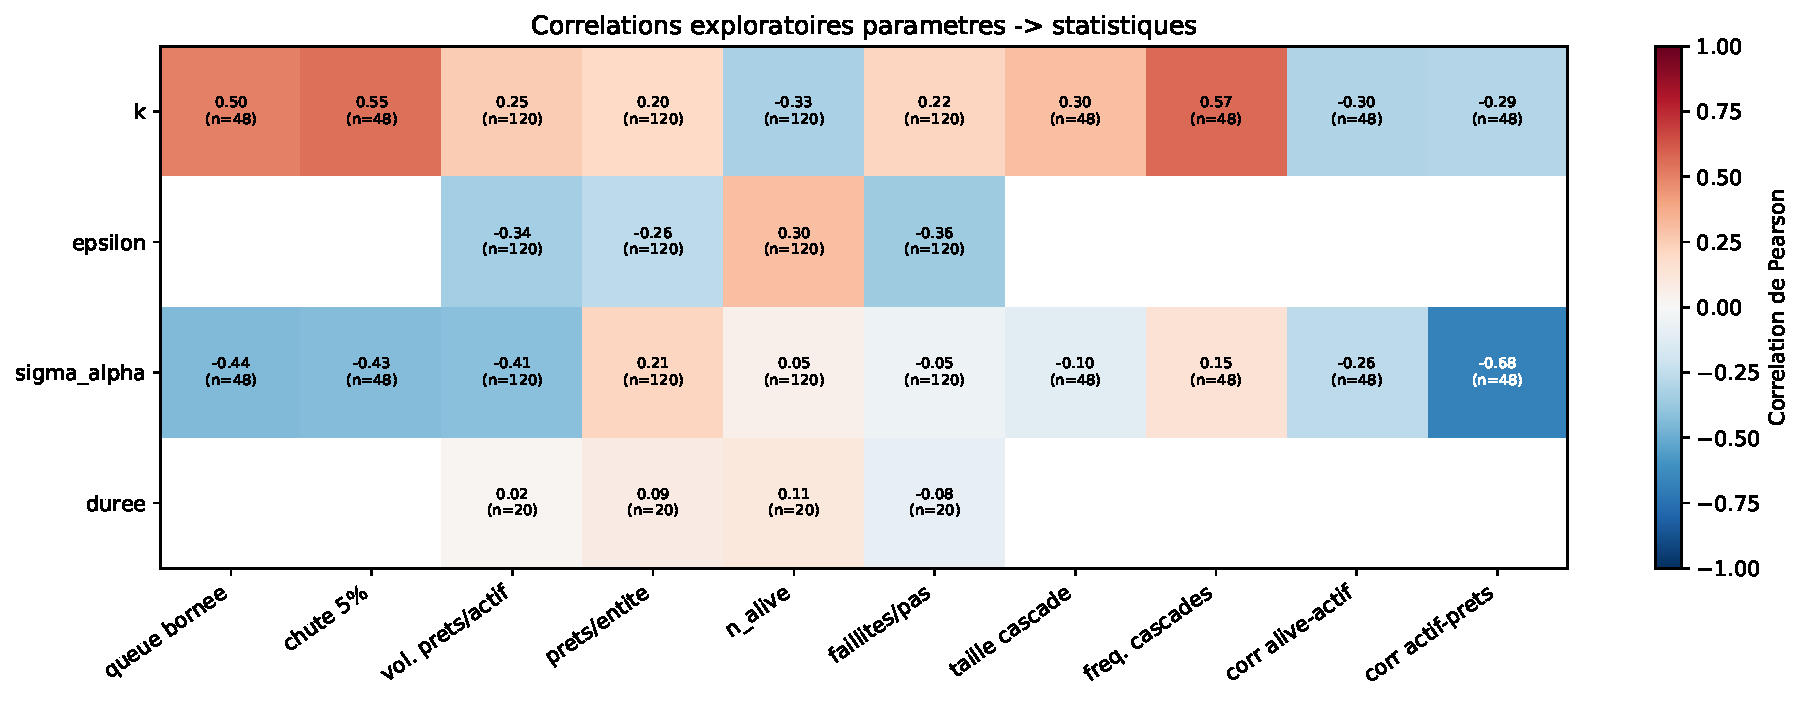
\includegraphics[width=0.98\linewidth]{figures/parameter_metric_correlations.pdf}
  \caption{Correlations exploratoires entre parametres de simulation et statistiques observees.}
\end{figure}

\section{Suite immediate}

La grande campagne de sensibilite doit donc etre construite autour de deux
centres :

\begin{enumerate}
  \item le point homogene sous-critique \(k=3\), pour mesurer quels parametres
  font apparaitre le regime ;
  \item le point homogene en regime \(k=4\), pour mesurer les sensibilites des
  criteres une fois le regime atteint.
\end{enumerate}

Les couplages prioritaires a tester sont \(k\) avec la depreciation exogene,
\(k\) avec \(\theta\), \(k\) avec \(\lambda\), et \(k\) avec l'heterogeneite
effective d'alpha, meme si cette derniere est exclue du scenario principal
homogene.

\end{document}
